\section{The canonical DR-plan}
\label{sec:DRP}
% In the problem of the optimal DR-Plan there is generally not a unique plan.
% % Indeed, we will prove a union of $N$ isostatic subgraphs will result in $N$ unique plans, but that at the $N^{\text{th}}$ level of the tree it will always be the same. Therefore, all choices of decomposition are in some sense equivalent. The theorem we seek to prove is thus:
% However, we will show that regardless of which children are chosen for the plan, so long as they satisfy the definition of an optimal DR-plan, the recombination will require solving of the same systems. Being the smallest such structure that offers this, the definition of an optimal DR-plan could be considered the canonical DR-plan.
% % To assist in showing this, we prove this core theorem throughout this section:

% In this section, we discuss 2D bar-joint graphs. All vertex weights are $2$, all edge weights are $1$, and constant $k= -{{3}\choose{2}}=-3$. Trivial graphs are a single vertex and empty set. Furthermore, 2D isostatic graphs must be connected.
% % The greatest density of a 2D isostatic graph is $-2$ (the vertex). The other disconnected part of the graph would need to have a density of $-1$, which is overconstrained and not possible in a isostatic graph (because there is no trivial graph with that density).

The NP-hardness of the DR-planning problem for 2D bar-joint graphs is partly the consequence of possibly exponential number of DR-plans. On the other hand, although the complete DR-plan is unique it could have large average fan-in and exponentially many nodes making it far from optimal.

In this section, we define a \dfn{canonical} plan to capture those aspects of an optimal DR-plan that mimic the uniqueness of a complete DR-plan, and we show that the nonunique parts do not affect optimality for independent (underconstrained or isostatic) graphs. Furthermore, we give an efficient \candrpcomplexity\ algorithm to find the canonical DR-plan of any independent graph. The definition is as follows:

\begin{definition}\label{def:canonical_drplan}
    The \dfn{canonical DR-plan} satisfies the following three properties:
    (1) it is a DR-plan;
    (2) children are rigid vertex-maximal proper subgraphs of the parent; and
    (3) if all pairs of rigid vertex-maximal proper subgraphs intersect trivially then all of them are children, otherwise take as children exactly two that intersect non-trivially.
\end{definition}



\subsection{Previous Work}
% \todo{We now briefly survey existing techniques for studying 2D qusecs,  many of which are \dfn{bar-joint} systems (Examples 1 and 2 above, see Sections \ref{sec:prelim}, \ref{sec:DRP}, and \ref{sec:recomb}), \dfn{body-hyperpin} systems (Example 4 and 5, see Section \ref{sec:bodypin}) or \dfn{pinned-line incidence} systems (Example 3, see Section \ref{sec:pinnedline}). The limitations of these techniques directly motivate the contributions of this paper.}
We now briefly survey existing techniques for detecting rigidity and creating DR-plans of 2D constraint systems. The limitations of these techniques directly motivate the contributions in this section.

\begin{enumerate}
    \item
    \header{Finding (vertex)-maximal generically rigid subsystems}
    Fast, graph-based algorithms exist (pebble-game \cite{Jacobs:1997:PG,lee2005finding}), for locating all maximal, \dfn{generically rigid} subsystems \seedefs. When the input itself is rigid, these algorithms do nothing, i.e., compute the identity function.

    However, both for self-similar or just aperiodic 2D qusecs, it is imperative to recursively decompose rigid systems into their rigid subsystems, down to the level of geometric primitives, in order to understand or design properties at all scales, such as \seedefs\ \dfn{rigidity}, \dfn{flexes}, distribution of \dfn{external stresses}, boundary conditions for \dfn{isostaticity}, as well as behavior under constraint variations.

    \item
    \header{Optimal Recursive Decomposition (DR-planning).}
    Recursive decomposition of geometric constraint systems has been formalized \cite{hoffman2001decompositionI,hoffman2001decompositionII} and well-studied \cite{jermann2006decomposition,sitharam2005combinatorial} as the \dfn {Decomposition-Recombination (DR-) planning} problem \seedefsprelim. For the abovementioned classes of 2D qusecs, generic rigidity is a combinatorial property and hence each level of the decomposition should, in principle, be achievable by a graph-based algorithm as in (1), without involving geometric information in the constraint system. Since many such decompositions can exist for a given constraint system, criteria defining desirable or optimal DR-plans and DR-planning algorithms were given in \cite{hoffman2001decompositionI}. An \dfn{optimal DR-plan} is one that minimizes the \dfn{size} \seedefsprelim, i.e., the maximum number of child subsystems of any parent system. Being exponential in the size, the complexity of solving the parent constraint system is overwhelmingly dominated by the complexity of solving the child systems.

    However, for general 2D qusecs that could be overconstrained, even when restricted to bar-joint systems, the optimal DR-planning problem was shown to be NP-hard \cite{lomonosov2004graph}.

    \item
    \header{DR-plans for special classes and with other criteria.}
    For a special class of 2D qusecs, namely \dfn{tree-decomposable} systems  \cite{fudos1997graph,owen1991algebraic,joan-arinyo2004revisiting}  common in computer aided mechanical design, (which includes ruler-and-compass and Henneberg-I constructible systems), all DR-plans turn out to be optimal. This satisfies the so-called \dfn{Church-Rosser} criterion, leading to highly efficient DR-planning algorithms. For general 2D qusecs, alternate criteria were suggested such as \dfn{cluster minimality} requiring parent systems to be composed of a minimal set of at least 2 rigid proper subsystems (i.e., no proper subset forms a rigid system); and \dfn{proper maximality}, requiring child subsystems to be maximal rigid proper subsystems of the parent system. \seedefsc.

    \indent
    While polynomial time algorithms were given to generate DR-plans meeting the cluster minimality criterion \cite{hoffman2001decompositionI}, no such algorithm is known for the latter criterion.
\end{enumerate}

\subsection{Theory}
In this section and in section~\ref{sec:recomb}, we deal exclusively with isostatic constraint systems. Any reference to some graph $G$ is assumed to be isostatic (i.e.\ well-constrained or $(k,l)$-tight).
% \sidenote{In this section, $G$ is always assumed to be isostatic.}



% This definition gives the canonical DR-plan a surprisingly strong Church-Rosser property.

Definition~\ref{def:canonical_drplan} gives the canonical DR-plan a surprisingly strong Church-Rosser property, which is made explicit in Theorem~\ref{theorem:main}, the main result of this section.

\begin{theorem}
\label{theorem:canonical_exists_and_is_optimal}
\label{theorem:canonical_is_optimal}
\label{theorem:main}
    A canonical DR-plan exists and any canonical DR-plan is optimal.
\end{theorem}


% \begin{theorem} \label{theorem:canonical_is_optimal}
%     \label{theorem:main}
%     Any canonical DR-plan is an optimal DR-plan.
% \end{theorem}

%The proof of this theorem is a direct consequence of the following  more general theorem.

%\begin{theorem}\label{theorem:main}
%Given an isostatic 2D bar-joint graph $G$ and ComDRP$(G)$, for all nodes $C$
%with children $C_1,\ldots,C_N$ preserve children according to the following rules.
%\begin{enumerate}
%    \item If $C_i \cap C_j$ is trivial then keep all $C_1,\ldots,C_N$ as children.
%    \item If $C_i \cap C_j$ is isostatic then select any two out of $C_1,\ldots,C_N$ as children.
%\end{enumerate}
%This is a canonical DR-plan.
%\end{theorem}


\begin{proof}
We show the existence of a canonical DR-plan by constructing it as follows:

Begin with $\comdrp{G}$ of a rigid 2D bar-joint graph $G$, for all nodes $C$ with children $C_1,\ldots,C_N$ keep children nodes according to the following rules:
\begin{enumerate}
   \item If $C_i \cap C_j$ is trivial then keep all $C_1,\ldots,C_N$ as children.
   \item If $C_i \cap C_j$ is rigid then select any two out of $C_1,\ldots,C_N$ as children.
\end{enumerate}

This directly satisfies properties 2 and 3 of a canonical DR-plan (see Definition~\ref{def:canonical_drplan}), because all the nodes in $\comdrp{G}$ are rigid vertex-maximal proper subgraphs. However, we still have to show property 1 (that this makes a DR-plan).
For rule (1), because we are beginning with a complete DR-plan, if we keep all the children it is still a DR-plan. For rule (2), we know that the union must be rigid as well and it cannot be anything other than $C$, otherwise we have found a larger rigid vertex-maximal proper subgraph.

If we begin with an isostatic graph, rigid can be replaced with isostatic throughout the construction and remain valid. The rigid proper subgraphs of an isostatic graph must be isostatic themselves.

Now we must show that a canonical DR-plan is optimal. The proof is by induction on the level of the plan; we show that following these rules always guarantees minimum fan-in at this level and does not increase fan-in on following levels.

 % We do this inductively on the l, beginning with the root node, showing that the rules are always the optimal choice.
% by discussing each rule and proving inductively that this is the optimal choice at each level of the DR-plan tree, starting with the root node.


% Now we show that this plan is optimal by considering the two cases. Observation \ref{lemma:union_intersection} shows that we do not have to consider anything other than the two cases stated in the construction.
 % the intersection of any two isostatic subgraphs can only result in trivial or isostatic subgraphs. Therefore, given $C$ and its isostatic vertex-maximal subgraphs $C_1,\ldots,C_N$, the are only two possibilities to consider. Either (1) subgraphs $C_i$ and $C_j$ have a trivial intersection, or (2) they have an isostatic intersection.





\medskip\noindent
\vemph{Rule 1:}
% If some pair is intersecting trivially, then in fact all pairs intersect trivially, thus all must be children by defn of canonical drplan
%
First, we claim that if the intersection is trivial all $C_1,\ldots,C_N$ must be children of $C$ in an optimal DR-plan. We do this by showing that no subset of the children can union to form $C$, thereby requiring all of them be included; because this is the only choice, it is the minimum fan-in any DR-plan could have for this node.
% must be optimal for this node.

Take the strict subset $S\subsetneq \{1,\ldots,N\}$ such that $U=\bigcup_{i\in S}{C_i}$ which we \vemph{assume} is isostatic. If $U\neq C$, then we just found a larger proper subgraph and the children were not vertex-maximal to begin with. So, it must be that $U=C$.
\usestwod
However, since $C_i \cap C_j$ is trivial then for $k\notin S$ we know, by Lemma \ref{lemma:combined_lemma}, point \ref{lemma:uc_intersection_makes_all_uc}, $U\cap C_k$ must be one or more trivial subgraphs. By definition of a DR-plan $C_k=C\cap C_k$ and we know that $U=C$ so $C_k=U\cap C_k$. Thus, $C_k$ is both one or more trivial subgraphs and a isostatic subgraph of $C$. Thus, the assumption is wrong and $U$ cannot be isostatic. As $C$ is isostatic, this means no proper subset of $C_1,\ldots,C_N$ can union to form $C$.

Furthermore, since a canonical DR-plan uses proper rigid \vemph{vertex-maximal} subgraphs as children, and because their pairwise intersection is trivial, it follows that any such node has at most as many children as a DR-plan without this restriction, because the union of the children have to contain all edges of the parent. Therefore, this is the optimal choice in this case.

\medskip\noindent
\vemph{Rule 2:} Second, we claim that if the intersection is isostatic, the choice of any two children will result in an optimal DR-plan.

If $C_i \cap C_j$ is isostatic, then, by Observation \ref{lemma:union_intersection}, $C_i \cup C_j$ is also isostatic. This means that, by Lemma \ref{lemma:combined_lemma}, point \ref{lemma:wc_intersection_makes_all_wc}, any two children of $C$ will union to $C$ itself. Thus, any two children can be chosen to make a canonical DR-plan.
% are potential choices for the optimal DR-plan as they all create equal fan-in (exactly two) at this level.

\newcommand{\induceonc}[1]{Idc\left(C,#1\right)}
\renewcommand{\induceonc}[1]{#1}
\newcommand{\iunion}[1]{\induceonc{I\cup\bigcup_{k\in S_N\setminus\{#1\}}{R_k}}}

However, to guarantee that any two are the \vemph{optimal} choice, it must ensure minimum fan-in over all descendants. Take the set $S_N=\{1,\dots,N\}$, then we call $I=\bigcap_{k\in S_N}{C_k}$ and $R_k=C\setminus C_k$. Suppose we select $i$ and $j$, where $i\neq j$, as the children. For convenience, we will assume all subgraphs are induced subgraphs on $C$. We know that $C=\induceonc{I\cup\bigcup_{k\in S_N}{R_k}}$ and $C_i=\iunion{i}$. The isostatic vertex-maximal subgraphs of $C_i$ are $(\iunion{i,1}),\ldots,(\iunion{i,i-1}),(\iunion{i,i+1}),\ldots,(\iunion{i,N})$ all of which intersect on isostatic subgraphs. So any two of these are viable children for $C_i$.
% Since
% \[C_i=Idc\left(C,I\cup\bigcup_{k\in S_N\setminus\{i\}}{R_k}\right)\]
% the children of $C_i$ will be
% \[Idc\left(C,I\cup\bigcup_{k\in S_N\setminus\{i,m\}}{R_k}\right)\]
% and
% \[Idc\left(C,I\cup\bigcup_{k\in S_N\setminus\{i,n\}}{R_k}\right)\]
% % $C_i=Idc\left(C,I\cup\bigcup_{k\in S_N\setminus\{i\}}{R_k}\right)$
% % the children of this node will be
% % $Idc\left(C,I\cup\bigcup_{k\in S_N\setminus\{i,m\}}{R_k}\right)$
% % and
% % $Idc\left(C,I\cup\bigcup_{k\in S_N\setminus\{i,n\}}{R_k}\right)$
% for arbitrary $m$ and $n$, where $i,j,m,n$ do not equal each other. \todo{Prove these are valid children? Or is this obvious?}
This continues for $N-1$ levels total, always with fan-in of two (the minimum possible), at which point every descendant of $C$ is some $\induceonc{I\cup R_k}$ for $k\in S_N$, with every $k$ appearing at least once. Thus, regardless of the choice of $C_i,C_j$, then their children, etc., the DR-plan has fan-in of two for every node for the next $N$ levels, at which point the nodes contain the same subgraphs. Therefore, the choice is optimal.
%
% \medskip\noindent
% This proof then applies to itself recursively to show that the fan-in of the children will also be minimum.
%
% -- say this at top `proof is by induction on the level of the dr=plan'
\end{proof}

This proof of this theorem relied on the following crucial observation and lemma. These will be used again in the application sections (\ref{sec:bodypin} and \ref{sec:pinnedline}) of the paper, with modifications to work for other types of qusecs.

\begin{observation*}\label{lemma:union_intersection}
If $F_i$ and $F_j$ are isostatic subgraphs of the same
isostatic graph $F$, \
then the following hold:
(1) $F_i\cup F_j$ is not trivial;
(2) $F_i\cup F_j$ is underconstrained if and only if $F_i\cap F_j$ is trivial;
(3) $F_i\cup F_j$ is isostatic if and only if $F_i\cap F_j$ is isostatic; and
(4) $F_i\cap F_j$ is not underconstrained.
\end{observation*}

Then the following key properties hold at the nodes of a canonical DR-plan.

\begin{lemma*}\label{lemma:combined_lemma}
Let $C$ be a node of a canonical DR-plan, with distinct children $C_i$ and $C_j$.
Then
\begin{enumerate}
    \item\label{lemma:wc_intersection_is_C}
    $C_i\cup C_j$ is isostatic if and only if $C_i\cup C_j = C$.

    \item\label{lemma:wc_intersection_makes_all_wc}
    If $C_i\cup C_j$ is isostatic, then $\forall k: C_i\cup C_k$ is isostatic. Alternatively, if $C_i\cup C_j=C$, then $\forall k: C_i\cup C_k=C$.

    \item\label{lemma:uc_intersection_makes_all_uc}
    If $C_i\cap C_j$ is trivial, then $\forall k: C_i\cap C_k$ is trivial.
\end{enumerate}
\end{lemma*}

\begin{remark}
The first item in the above lemma generalizes to the union of any number of children, $C_1,\ldots,C_k$, resulting in the desirable property of \dfn{Cluster Minimality}, defined in \cite{hoffman2001decompositionI} holding for these canonical-optimal DR-plans.
\end{remark}






% \begin{figure*}\centering
% \begin{subfigure}{.3\linewidth}\centering
%     % \newcommand{\tedge}[5]{\draw[#3] (#1)-- node[e, #5] (e#4) {#4} (#2)}

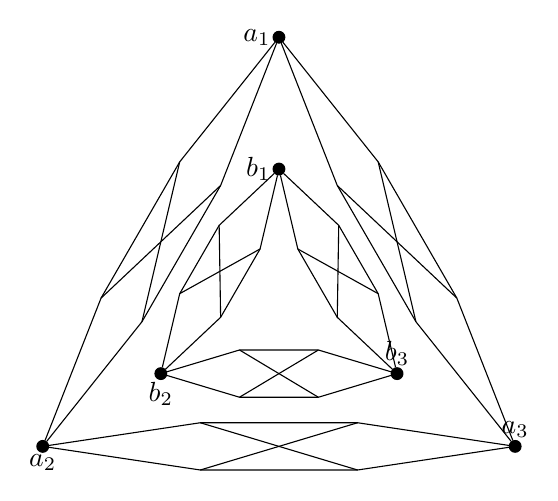
\begin{tikzpicture}[scale=3]
    \tikzstyle{v}=[draw, circle, minimum size=0.75cm]
    \tikzstyle{c}=[draw, circle, inner sep=1.5, fill=black]
    \tikzstyle{e}=[]

    \node[circle,fill=white,inner sep=7] (center) at (0,0-.125-.1) {};

    \node[c] (v1) at (0,0.866) [label={left,inner sep=.555}:$a_1$]{};
    \node[c] (v2) at (-1,-0.866) [label={below,inner sep=.555}:$a_2$]{};
    \node[c] (v3) at (1,-0.866) [label={above,inner sep=.555}:$a_3$]{};

    \node[c] (v4) at (0,0.433-.125) [label={left,inner sep=.555}:$b_1$]{};
    \node[c] (v5) at (-0.5,-0.433-.125) [label={below,inner sep=.555}:$b_2$]{};
    \node[c] (v6) at (0.5,-0.433-.125) [label={above,inner sep=.555}:$b_3$]{};

    \tedge{v1}{v2}{solid}{}{};
    \tedge{v1}{v3}{solid}{}{};
    \tedge{v2}{v3}{solid}{}{};

    \tedge{v4}{v5}{solid}{}{};
    \tedge{v4}{v6}{solid}{}{};
    \tedge{v5}{v6}{solid}{}{};


    \tedge{v1}{v4}{solid}{}{};
    \tedge{v2}{v5}{solid}{}{};
    \tedge{v3}{v6}{solid}{}{};


    \tedge{v4}{center}{dashed}{}{};
    \tedge{v5}{center}{dashed}{}{};
    \tedge{v6}{center}{dashed}{}{};


    % sin(30deg) = 0.5
    % cos(30deg) = 0.866

    % o/i -> outside/inside triangle
    % b/l/r -> bottom/left/right edge of triangle

    \coordinate (ob0) at (-0.333,-0.866-0.1);
    \coordinate (ob1) at (0.333,-0.866-0.1);
    \coordinate (ob2) at (-0.333,-0.866+0.1);
    \coordinate (ob3) at (0.333,-0.866+0.1);
    \draw (v2) -- (ob0) -- (ob1) -- (v3);
    \draw (v2) -- (ob2) -- (ob3) -- (v3);
    \draw (ob0) -- (ob3);
    \draw (ob2) -- (ob1);

    \draw[rotate around={60:(-1,-0.866)}] (v2) -- (-0.333,-0.766) -- (0.333,-0.766) -- (v1);
    \draw[rotate around={60:(-1,-0.866)}]  (v2) -- (-0.333,-0.966) -- (0.333,-0.966) -- (v1);
    \draw[rotate around={60:(-1,-0.866)}]  (-0.333,-0.766) -- (0.333,-0.966);
    \draw[rotate around={60:(-1,-0.866)}]  (-0.333,-0.966) -- (0.333,-0.766);

    \draw[rotate around={-60:(1,-0.866)}] (v3) -- (0.333,-0.766) -- (-0.333,-0.766) -- (v1);
    \draw[rotate around={-60:(1,-0.866)}]  (v3) -- (0.333,-0.966) -- (-0.333,-0.966) -- (v1);
    \draw[rotate around={-60:(1,-0.866)}]  (-0.333,-0.766) -- (0.333,-0.966);
    \draw[rotate around={-60:(1,-0.866)}]  (-0.333,-0.966) -- (0.333,-0.766);




    \coordinate (ib0) at (-0.167,-0.433-.125-0.1); %(-.167,-.658)
    \coordinate (ib1) at (0.167,-0.433-.125-0.1); %(.167,-.658)
    \coordinate (ib2) at (-0.167,-0.433-.125+0.1);%(-.167,-.458)
    \coordinate (ib3) at (0.167,-0.433-.125+0.1);%(.167,-.458)
    \draw (v5) -- (ib0) -- (ib1) -- (v6);
    \draw (v5) -- (ib2) -- (ib3) -- (v6);
    \draw (ib0) -- (ib3);
    \draw (ib2) -- (ib1);

    \draw[rotate around={60:(-0.5,-0.558)}] (v5) -- (-.167,-.658) -- (.167,-.658) -- (v4);
    \draw[rotate around={60:(-0.5,-0.558)}]  (v5) -- (-.167,-.458) -- (.167,-.458) -- (v4);
    \draw[rotate around={60:(-0.5,-0.558)}]  (-.167,-.658) -- (.167,-.458);
    \draw[rotate around={60:(-0.5,-0.558)}]  (-.167,-.458) -- (.167,-.658);

    \draw[rotate around={-60:(0.5,-0.558)}] (v6) -- (.167,-.658) -- (-.167,-.658) -- (v4);
    \draw[rotate around={-60:(0.5,-0.558)}]  (v6) -- (.167,-.458) -- (-.167,-.458) -- (v4);
    \draw[rotate around={-60:(0.5,-0.558)}]  (-.167,-.658) -- (.167,-.458);
    \draw[rotate around={-60:(0.5,-0.558)}]  (-.167,-.458) -- (.167,-.658);
% \newcommand{\tedge}[5]{\draw[#3] (#1)-- node[e, #5] (e#4) {#4} (#2)}

    % \draw (-1,-0.866) -- (-0.333,-0.966);

\end{tikzpicture}

%     \caption{}\label{fig:c2c3ofk33s:a}
% \end{subfigure}%
% \begin{subfigure}{.7\linewidth}\centering
%     % \newcommand{\tedge}[5]{\draw[#3] (#1)-- node[e, #5] (e#4) {#4} (#2)}

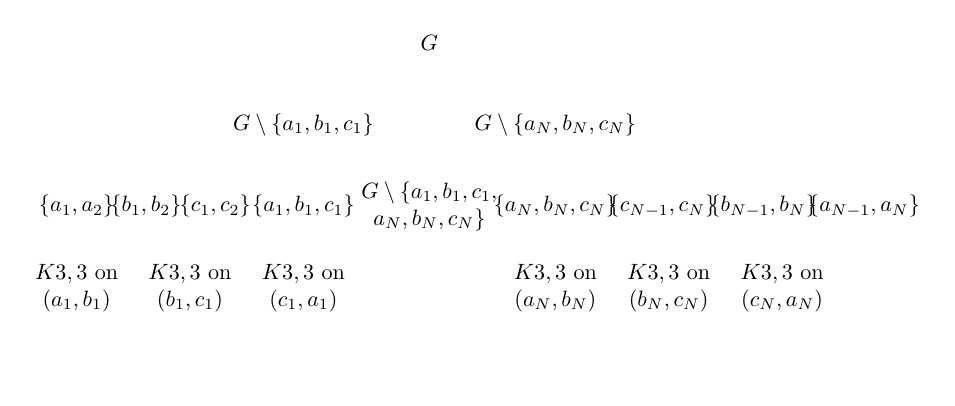
\begin{tikzpicture}[scale=.8, transform shape]
    \tikzstyle{v}=[draw, circle, minimum size=0.75cm, font=\footnotesize]
    % \tikzstyle{b}=[draw, font=\footnotesize]
    \tikzstyle{b}=[align=center]
    \tikzstyle{e}=[]

    \node[b] (c0) at (0,0*1.3) {$G$};
    \node[b] (c1a) at (-2,-1*1.3) {$G\setminus\{a_1,b_1,c_1\}$};
    \node[b] (c1b) at (2,-1*1.3) {$G\setminus\{a_N,b_N,c_N\}$};
    \node[b] (c2b) at (0,-2*1.3) {$G\setminus\{a_1,b_1,c_1,$ \\ $a_N,b_N,c_N\}$};
    \node[b] (c2a) at (-2,-2*1.3) {$\{a_1,b_1,c_1\}$};
    \node[b] (c2c) at (2,-2*1.3) {$\{a_N,b_N,c_N\}$};
    \node[b] (c2ab1) at (-5.6,-2*1.3) {$\{a_1,a_2\}$};
    \node[b] (c2ab2) at (-4.5,-2*1.3) {$\{b_1,b_2\}$};
    \node[b] (c2ab3) at (-3.4,-2*1.3) {$\{c_1,c_2\}$};
    \node[b] (c2bc1) at (6.9,-2*1.3) {$\{a_{N-1},a_N\}$};
    \node[b] (c2bc2) at (5.3,-2*1.3) {$\{b_{N-1},b_N\}$};
    \node[b] (c2bc3) at (3.7,-2*1.3) {$\{c_{N-1},c_N\}$};

    \node[b] (ab1k33) at (-5.6,-3*1.3) {$K3,3$ on \\ $(a_1,b_1)$};
    \node[b] (bc1k33) at (-7.6/2,-3*1.3) {$K3,3$ on \\ $(b_1,c_1)$};
    \node[b] (ca1k33) at (-2,-3*1.3) {$K3,3$ on \\ $(c_1,a_1)$};

    \node[b] (abNk33) at (2,-3*1.3) {$K3,3$ on \\ $(a_N,b_N)$};
    \node[b] (bcNk33) at (7.6/2,-3*1.3) {$K3,3$ on \\ $(b_N,c_N)$};
    \node[b] (caNk33) at (5.6,-3*1.3) {$K3,3$ on \\ $(c_N,a_N)$};


    \node[b] (c3a) at (-2,-4*1.3) {};
    \node[b] (c3b) at (2,-4*1.3) {};


    \tedge{c0}{c1a}{solid}{}{};
    \tedge{c0}{c1b}{solid}{}{};

    \tedge{c1a}{c2ab1}{solid}{}{};
    \tedge{c1a}{c2ab2}{solid}{}{};
    \tedge{c1a}{c2ab3}{solid}{}{};
    \tedge{c1a}{c2a}{solid}{}{};
    \tedge{c1a}{c2b}{solid}{}{};

    \tedge{c1b}{c2bc1}{solid}{}{};
    \tedge{c1b}{c2bc2}{solid}{}{};
    \tedge{c1b}{c2bc3}{solid}{}{};
    \tedge{c1b}{c2b}{solid}{}{};
    \tedge{c1b}{c2c}{solid}{}{};

    \tedge{c2a}{ab1k33}{solid}{}{};
    \tedge{c2a}{bc1k33}{solid}{}{};
    \tedge{c2a}{ca1k33}{solid}{}{};
    \tedge{c2c}{abNk33}{solid}{}{};
    \tedge{c2c}{bcNk33}{solid}{}{};
    \tedge{c2c}{caNk33}{solid}{}{};

    \tedge{c2b}{c3a}{dashed}{}{};
    \tedge{c2b}{c3b}{dashed}{}{};
\end{tikzpicture}

%     \caption{}\label{fig:c2c3ofk33s:b}
% \end{subfigure}

% \caption{(\ref{fig:c2c3ofk33s:a}) A doublet ($C_2 \times C_3$) with each edge of the triangles replaced by a $K_{3,3}$. This pattern continues inwards for a total of $N$ triangles, indicated by the dashed lines. (\ref{fig:c2c3ofk33s:b}) Most of the DR-plan of this graph, omitting further decomposition of $K_{3,3}$ subgraphs into the separate 9 edges and of edges into the component nodes. $G\setminus\{a_i,b_i,c_i\}$ is shorthand for $G$ difference those nodes and all of the nodes in the corresponding $K_{3,3}$ subgraphs. The dashed lines indicated that this exact structure is repeated.}
% \label{fig:c2c3ofk33s}
% \end{figure*}


% \FigInit
%     {(\ref{fig:c2c3ofk33s:a}) A doublet ($C_2 \times C_3$) with each edge of the triangles replaced by a $K_{3,3}$. This pattern continues inwards for a total of $N$ triangles, indicated by the dashed lines. (\ref{fig:c2c3ofk33s:b}) Most of the DR-plan of this graph, omitting further decomposition of $K_{3,3}$ subgraphs into the separate 9 edges and of edges into the component nodes. $G\setminus\{a_i,b_i,c_i\}$ is shorthand for $G$ difference those nodes and all of the nodes in the corresponding $K_{3,3}$ subgraphs. The dashed lines indicated that this exact structure is repeated.}
%     {fig:c2c3ofk33s}
% \FigTwoSubfigWithWidth
%     {.3}
%     {img/epsfromtikz/c2c3_of_k33s-0}
%     {}
%     {fig:c2c3ofk33s:a}
%     %
%     {.7}
%     {img/epsfromtikz/c2c3_of_k33s-1}
%     {}
%     {fig:c2c3ofk33s:b}


\ClearMyMinHeight
\SetMyMinHeight{.3}{img/epsfromtikz/c2c3_of_k33s-0}
\SetMyMinHeight{.7}{img/epsfromtikz/c2c3_of_k33s-1}

\begin{figure*}\centering%
    %
    \begin{subfigure}{0.3\linewidth}\centering
        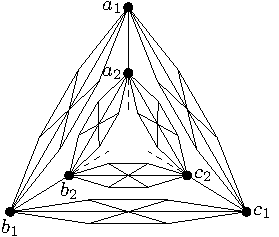
\includegraphics[height=\myMinHeight]{img/epsfromtikz/c2c3_of_k33s-0}
        \caption{}\label{fig:c2c3ofk33s:a}
    \end{subfigure}%
    %
    \hfill
    \begin{subfigure}{0.7\linewidth}\centering
        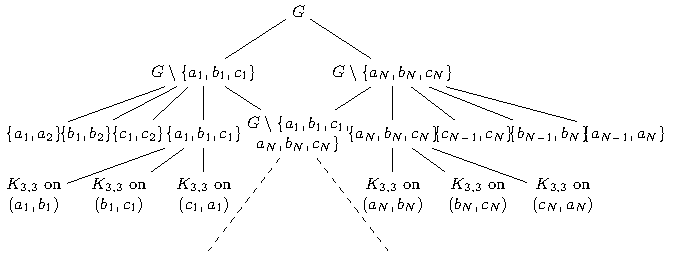
\includegraphics[height=\myMinHeight]{img/epsfromtikz/c2c3_of_k33s-1}
        \caption{}\label{fig:c2c3ofk33s:b}
    \end{subfigure}%
    %
    \caption{(\ref{fig:c2c3ofk33s:a}) A doublet ($C_2 \times C_3$) with each edge of the triangles replaced by a $K_{3,3}$. This pattern continues inwards for a total of $N$ triangles, indicated by the dashed lines. (\ref{fig:c2c3ofk33s:b}) Most of the DR-plan of this graph, omitting further decomposition of $K_{3,3}$ subgraphs into the separate 9 edges and of edges into the component nodes. $G\setminus\{a_i,b_i,c_i\}$ is shorthand for $G$ difference those nodes and all of the nodes in the corresponding $K_{3,3}$ subgraphs. The dashed lines indicated that this exact structure is repeated.}
    \label{fig:c2c3ofk33s}
\end{figure*}%




\myexample
\textsl{[DR-Plan for self-similar structure]}
This section details the decomposition of the graph in Figure \ref{fig:c2c3ofk33s}. The graph $G$ has only two isostatic vertex-maximal subgraphs, $G$ without the outermost triangle composed of $K_{3,3}$ graphs (triangle $1$) and $G$ without the inner triangle $N$. These intersect on $G$ without triangle $1$ and $N$ which is clearly isostatic. As explained in the proof of Theorem \ref{theorem:main} since there are only 2 possible children, their intersection must be a node 2 levels below the parent. Just as expected, it is on the third level, as it is a child of both of $G$'s children. Furthermore, it intersects trivially with the edges that connect triangle $1$ and $N$ to $2$ and $N-1$, respectively; these necessarily intersect with triangle $1$ and $N$ themselves trivially (by Theorem \ref{theorem:main}, part 1) making all of these children. The triangles then decompose into their constituent $K_{3,3}$ graphs, which then decompose into 9 edges.

Now, the self-similar nature of the graph is clear; $G$ without triangle $1$ and $N$ has the same structure, and thus the same pattern is repeated until only triangle $(N+1)/2$ remains in the case that $N$ is odd, or until only triangles $N/2$ and $N/2+1$ remain if $N$ is even.


% \begin{example}
%     In
% \end{example}




% \subsection{Extensions}
% This framework immediately pushes through for body-pin systems via a simple reduction. If there are $N$ pins on a body, it can be represented as a 2-tree with $N$ vertices, each corresponding to a pin, making sure to select edge distances such that the distance between pins is preserved. E.g.\ a body with two pins is an edge, three pins is a triangle, etc. Any bodies that share a pin now intersect on their vertex that corresponds to that pin. Now we have a bar-joint representation of the body-pin system in 2D and all proofs follow.

% With more effort, it can be shown that pinned line-incidence systems can also use this framework. This is done in section \ref{XXX}.


\subsection{Algorithm}



% \ClearMyMinHeight
% \SetMyMinHeight{.4}{img/epsfromtikz/demo_graph}
% \SetMyMinHeight{.3}{img/epsfromtikz/demo_graph_comdrp}
% \SetMyMinHeight{.3}{img/epsfromtikz/demo_graph_candrp}

% \begin{figure*}\centering%
%   %
%   \begin{subfigure}{0.4\linewidth}\centering
%     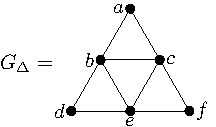
\includegraphics[height=\myMinHeight]{img/epsfromtikz/demo_graph}
%     \caption{}\label{fig:demo_graph:graph}
%   \end{subfigure}%
%   %
%   \hfill
%   \begin{subfigure}{0.3\linewidth}\centering
%     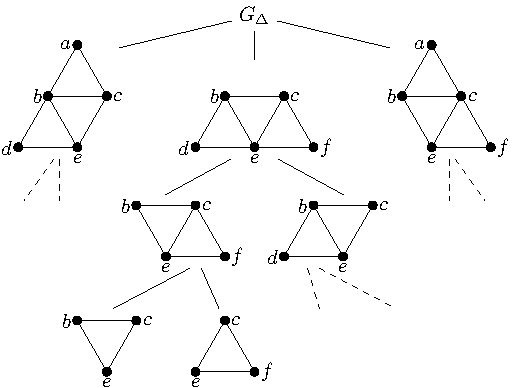
\includegraphics[height=\myMinHeight]{img/epsfromtikz/demo_graph_comdrp}
%     \caption{}\label{fig:demo_graph:comdrp}
%   \end{subfigure}%
%   %
%   \hfill
%   \begin{subfigure}{0.3\linewidth}\centering
%     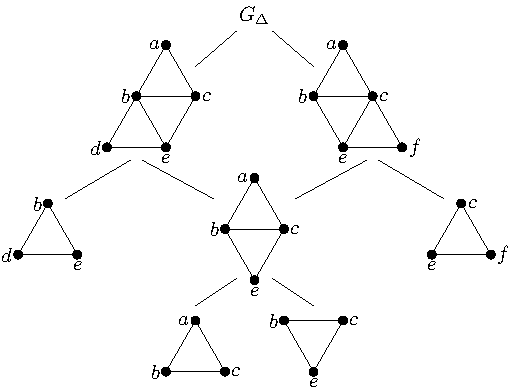
\includegraphics[height=\myMinHeight]{img/epsfromtikz/demo_graph_candrp}
%     \caption{}\label{fig:demo_graph:candrp}
%   \end{subfigure}%
%   %
%   \caption{(\ref{fig:demo_graph:graph}) A simple graph, $G_{\Delta}$, used to illustrate concepts throughout this and the next section. (\ref{fig:demo_graph:comdrp}) The complete DR-plan of $G_{\Delta}$, i.e.\ $ComDRP(G_{\Delta})$. Dashed lines indicate that the children repeat the same pattern as the others shown on this level. The children of triangles (3 edges) are omitted. (\ref{fig:demo_graph:candrp}) The canonical DR-plan of $G_{\Delta}$, which is optimal (see Section~\ref{sec:DRP}), i.e.\ $OptDRP(G_{\Delta})$. The children of triangles or omitted.}
%   \label{fig:demo_graph}
% \end{figure*}%

% \begin{figure*}\centering%
%   %
%   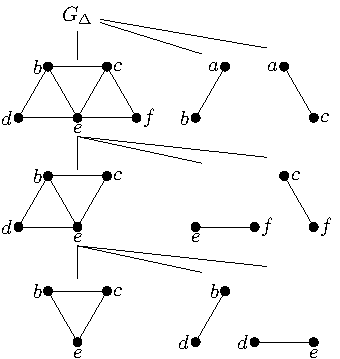
\includegraphics[width=0.3\linewidth]{img/epsfromtikz/demo_graph_candrp_seq}
%   \caption{The sequential canonical DR-plan of $G_{\Delta}$ from Figure~\ref{fig:demo_graph:graph}, which is optimal (as explained in the proof of Theorem~\ref{theorem:algo_complexity}). The children of the triangle are omitted. Compare to to the typical canonical DR-plan shown in Figure~\ref{fig:demo_graph:candrp}. Also, note that the bottom-left node, the triangle $bce$, is the intersection of the 3 children of $G_{\Delta}$ in $ComDRP(G_{\Delta})$, shown in Figure~\ref{fig:demo_graph:comdrp}.}
%   \label{fig:demo_graph:candrpseq}
% \end{figure*}%
\begin{figure*}\centering%
  %
  \includegraphics[width=0.3\linewidth]{img/svg/3xc2c3_candrp_seq}
  \caption{The sequential canonical DR-plan of $G_{demo}$ from Figure~\ref{fig:demo_graph:graph}, which is optimal (as explained in the proof of Theorem~\ref{theorem:algo_complexity}). The children of the triangle are omitted. Compare to to the typical canonical DR-plan shown in Figure~\ref{fig:demo_graph:candrp}. Also, note that the bottom-left node, the triangle, is the intersection of the 3 children of $G_{demo}$ in $ComDRP(G_{demo})$, shown in Figure~\ref{fig:demo_graph:comdrp}.}
  \label{fig:demo_graph:candrpseq}
\end{figure*}%

\begin{theorem}\label{theorem:algo_complexity}
    There exists an \candrpcomplexityv\ algorithm to find a canonical DR-plan for any 2D isostatic bar-joint graph.
\end{theorem}

\begin{proof}
The first step of the algorithm, which we call $CanDRP(G)$, is finding the isostatic vertex-maximal proper subgraphs of the input isostatic graph $G$. Do this by first dropping arbitrary edge $e$ from the edge set and running the pebble game algorithm \cite{Jacobs:1997:PG} on this subgraph, which is $O(|V|^2)$. The output of this will be a list of component-candidates. Then run the Frontier algorithm \cite{hoffman2001decompositionII} \cite{lomonosov2004graph} ($O(|V|)$) on each candidate along with edge $e$, which will find the minimal subgraph $D$ that contains the candidate and $e$. If $D=G$, move the candidate (before adding $e$) to the true-component list and remove it from the candidate-component list. If $D\subsetneq G$, remove all candidates that are subgraphs of $D$ from the candidate-component list and add $D$ back to the list. Continue with the next candidate. When you exhaust the candidates, move to the next step.

Test the intersection of any two of the true-components. If the intersection is trivial, the entire list become the children; recursively apply the algorithm to each child. If the intersection is non-trivial (necessarily isostatic), immediately compute the sequential decomposition down to $I=\bigcap_{k=1}^{N}{C_k}$. The root of this idea is discussed in detail in the proof of Theorem \ref{theorem:main}. We construct a DR-plan whose node set is the same as that of a canonical/optimal DR-plan. Begin with the parent $C$. Its children will be $S_1$ and $CanDRP(T_1)$, where $S_1=C\setminus R_1$ and $T_1$ is $R_1$ plus all incident edges (observe that these edges will add nodes from $I$ and that $T_1$ is underconstrained so it will be a forest and each root becomes a child of $C$). The children of $S_1$ will be $S_2$ and $CanDRP(T_2)$, where $S_2=C\setminus (R_1\cup R_2)$ and $T_2$ is $R_2$ plus all incident edges. And so on. At $N$ levels down, the children will be $S_N=I$ and $CanDRP(T_N)$, where $T_N$ is $R_N$ plus all incident edges. Apply the algorithm recursively to both children. See Figure~\ref{fig:demo_graph:candrpseq} for an example. \todo{should this more elaborate discussion be moved outside the proof?}

The previous discussion was a detailed explanation with an implied efficient method to solve for the case of non-trivial intersections, which avoids recomputation of the isostatic components of $C$. This stage of the algorithm could be stated more succinctly:
if the intersection is trivial, recursively apply $CanDRP$ to the entire list of true-components and set the resulting trees as the children. Else, the intersection is non-trivial, and the children of the node are $CanDRP(C_1)$ and $CanDRP(T)$, where $C_1$ is the first true-component of the parent $C$ (chosen arbitrarily, could be any child) and $T$ is the underconstrained graph formed from $C\setminus C_1$ plus all incident edges (also adding the associated nodes in $C_1$).

% Although the nodes containing $R_1,\ldots,R_N$ are underconstrained, simply take the children to be the roots of the forest

The reason for this construction is that it makes analysis of the algorithm convenient. The result of the algorithm is DR-plan that is a tree with no duplicate nodes. The leaves of this tree will be exactly the edges of this graph. Therefore, the number of nodes in the tree is $O(|E|)$ which, for isostatic input graphs, is $O(|V|)$.

Therefore, the complexity of the algorithm as a whole is $O(|V|^3)$.
%
% \note In the best case, this can be $O(V^2)$ if the graph is a 2-tree
\end{proof}


% \begin{proof}
% The first step of the algorithm is finding the isostatic vertex-maximal proper subgraphs of the input isostatic graph $G$. Do this by first dropping arbitrary edge $e$ from the edge set and running the pebble game algorithm \cite{Jacobs:1997:PG} on this subgraph, which is $O(|V|^2)$. The output of this will be a list of component-candidates. Then run the Frontier algorithm \cite{hoffman2001decompositionII} \cite{lomonosov2004graph} ($O(|V|)$) on each candidate along with edge $e$, which will find the minimal subgraph $D$ that contains the candidate and $e$. If $D=G$, move $D$ to the true-component list and remove the candidate from the candidate-component list. If $D\subsetneq G$, check the union of $D$ with the all items in the true-component list; if the union is isostatic, halt and output just these two components as children. Otherwise, remove all candidates that are subgraphs of $D$ from the candidate-component list and add $D$. Continue with the next candidate. If you exhaust the candidates, output the entire true-component list.

% %on the children
% This is run recursively on each node. If you use dynamic programming to store the decompositions of each component, it prevents repetition of work (done by using the DAG representation of the DR-plan). In this case you will have to do work on no more than $O(|V|)$ nodes that get smaller at each level.

% Thus, the running time is at most $O(|V|^3)$. \todo{does this amortize correctly?}

% It's a tree in only trivial case -> O(V), always order of leaves
% If its isostatic intersection, we do the sequential extension,intersections only done once.

% inductively. The number of nodes at this level will e more than the total. Number of leaves (terminals for dag) is at most the number of edges

% \end{proof}

% \begin{proof}
% The first step of the algorithm to find an optimal DR-plan is the most difficult --- to find the wellconstrained vertex-maximal proper subgraphs of the input wellconstrained graph. There are two approaches: (1) the bottom-up approach, using the Frontier algorithm \cite{Oung:2001:FFE:376957.376995} to grow these components from single vertices; and (2) the top-down approach, using the pebble game algorithm \cite{Jacobs:1997:PG} on each node and taking the largest components that are not subgraphs of any larger ones. After the subgraphs have been found, it is a straightforward application of the theory. If the intersection of any two of the subgraphs is wellconstrained, then take those two to be children of the graph. Otherwise, all the subgraphs are the children. Apply recursively to the children. This naturally terminates when you reach trivial subgraphs. The complexity of this depends on the algorithm for finding children (both are polynomial) and the depth of the plan (the deeper the plan, i.e.\ the smaller the max fan-in, the longer the running time). \todo{Think more about complexity.}
% \end{proof}

\begin{remark}
    While the canonical DR-plan is optimal only if the input graph is independent, if there are only $k$ overconstraints for some fixed $k$, we can still find the optimal DR-plan. However, the time complexity is exponential in $k$.
\end{remark}

\begin{conjecture}
\label{conj:mfaisoptimal}
    The Modified Frontier Algorithm (MFA)~\cite{lomonosov2004graph} finds a canonical, and hence optimal, DR-plan.
\end{conjecture}

The difficulty of proving Conjecture~\ref{conj:mfaisoptimal} arises from the fact that MFA is a bottom-up algorithm, involving complex datastructures. However, such a proof, even if it exists, would not be possible without the new notion of a canonical DR-plan at hand. The intuition for this conjecture comes from the similarity of the DR-plan generated by MFA to that of the sequential decomposition described in the proof of Theorem~\ref{theorem:algo_complexity}. The strength of MFA compared to other DR-planning algorithms is illustrated in the paper~\cite{lomonosov2004graph}. While MFA also offers complexity $O(n^3)$, it does not guarantee optimality.
